%% LyX 2.0.3 created this file.  For more info, see http://www.lyx.org/.
%% Do not edit unless you really know what you are doing.
\documentclass[11pt,spanish]{article}
\usepackage{mathptmx}
\usepackage[T1]{fontenc}
\usepackage[latin1]{inputenc}
\usepackage[a4paper]{geometry}
\geometry{verbose,tmargin=2cm,bmargin=2cm,lmargin=2cm,rmargin=2cm}
\usepackage{float}
\usepackage{units}
\usepackage{amstext}
\usepackage{graphicx}
\PassOptionsToPackage{normalem}{ulem}
\usepackage{ulem}

\makeatletter
%%%%%%%%%%%%%%%%%%%%%%%%%%%%%% User specified LaTeX commands.
%%\usepackage{SEART}

%TCIDATA{TCIstyle=article/art4.lat,SEART,SEART}

%TCIDATA{Created=Mon Aug 20 21:09:02 2001}
%TCIDATA{LastRevised=Tue May 14 08:11:44 2002}
%% \input{tcilatex}

\makeatother

\usepackage{babel}
\addto\shorthandsspanish{\spanishdeactivate{~<>}}

\begin{document}
\begin{center}
\textsc{\large Física 2 (Físicos) - Cátedra Diana Skigin}
\par\end{center}{\large \par}
\begin{center}
\textsc{\large Segundo Cuatrimestre de 2020}
\par\end{center}{\large \par}

\begin{center}
\textsc{\large Guía 5: Interferencia y Difracción}
\par\end{center}{\large \par}

\textsc{Interferencia}

\begin{enumerate}
\item Diga qué entiende por luz cuasi monocromática y dé algunos ejemplos.
\item ¿Bajo qué condiciones se puede decir que dos fuentes son coherentes?
¿Es posible observar interferencia de la luz proveniente de dos tubos
fluorescentes? ¿Por qué? Diga cuándo es posible observar interferencia.
\item Diga qué entiende por interferómetro por división de frente de onda.
Mencione los más representativos, haga un esquema de cada uno de ellos
e indique sus parámetros característicos.
\item ~
\begin{enumerate}
\item En el experimento de Young, ¿cuál es el lugar geométrico de los puntos
que reciben ondas con la misma diferencia de fases?
\item Si en un experimento de Young la pantalla de observación está lo suficientemente
alejada de las ranuras, ¿qué aspecto tienen las franjas de interferencia?
\end{enumerate}
\item Sea una fuente monocromática ($\lambda=$5500 Å), y un dispositivo
de Young de las siguientes características: 
Distancia entre ranuras: $s=3,3$ mm. 
Distancia de las ranuras a la pantalla: $D=3$ m.
\begin{figure}[H]
\centering{}\includegraphics[clip,scale=0.25]{ej5-5}
\end{figure}
\begin{enumerate}
\item Calcular la interfranja $i$.
\item Detrás de una de las ranuras se coloca una lámina de vidrio de caras
paralelas y planas ($e=0,01$ mm) (ver figura). Determinar el sentido
de desplazamiento de las franjas y la fórmula que da la expresión
de dicho desplazamiento. Sabiendo que las franjas se han desplazado
4,73 mm, dar el valor del índice de refracción del vidrio. ¿Puede
detectar dicho corrimiento con una fuente monocromática? ¿Y con una
policromática?
\end{enumerate}
\item ¿Cómo cambia el experimento de Young si la fuente luminosa no está
simétricamente situada respecto de la ranura, o si, por algún motivo,
las ondas que llegan a las mismas tienen un cierto desfasaje? ¿Cómo
puede detectar dicho corrimiento?
\item Se tiene el dispositivo para producir interferencia que indica la
figura. La fuente puntual monocromática de longitud de onda $\lambda$
(linealmente polarizada en el eje $z$, con amplitud $E_{0}$), ilumina
dos rendijas separadas por una distancia $a$. La fuente está centrada
respecto de las rendijas y se encuentra a una distancia $L_{0}$ de
las mismas. A la izquierda de las rendijas hay dos medios distintos;
sobre el eje $x$ es $n_{1}$, y debajo del eje $x$ es $n_{2}$ ($n_{2}>n_{1}$);
a la derecha de las rendijas el índice es $n_{1}$ solamente. A continuación
de la rendija 2 se coloca una lámina polarizadora cuyo eje de transmisión
forma un ángulo $\alpha$ con el eje $z$. 
\begin{description}
\item [{Datos:}] $a$, $n_{2}$, $n_{1}$, $E_{0}$, $L_{0}$, $L$.
\begin{figure}[H]
\centering{}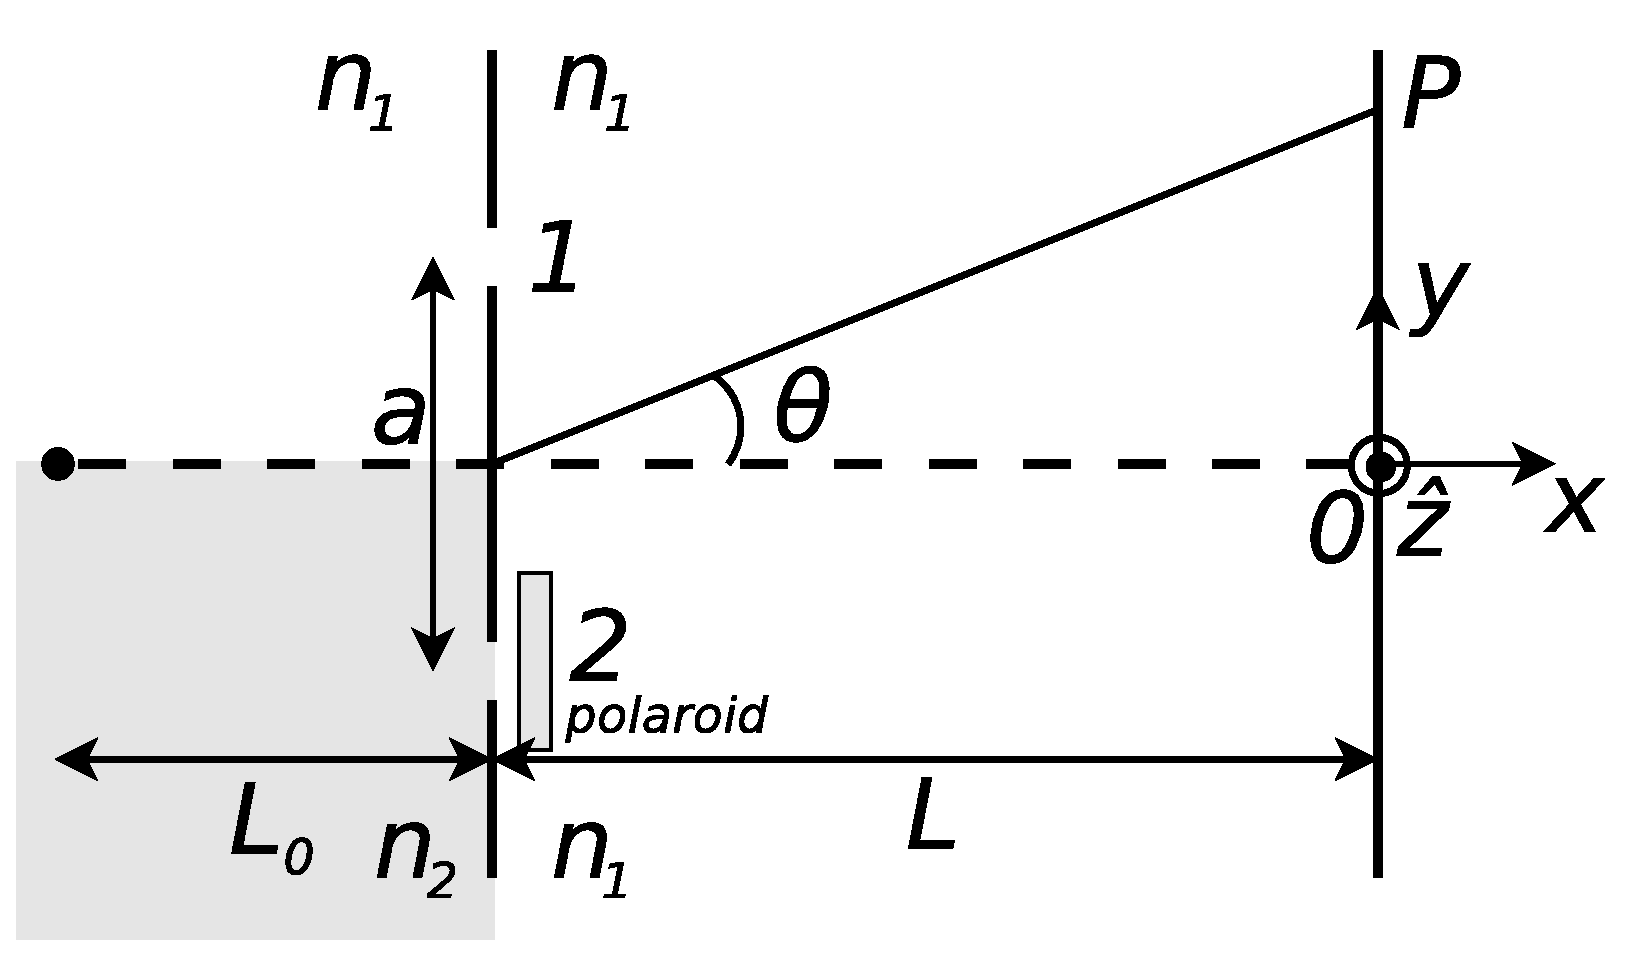
\includegraphics[clip,scale=0.3]{ej5-7}
\end{figure}
\end{description}
\begin{enumerate}
\item ¿Qué efecto produce en el patrón de interferencia la diferencia de
medios? Explique.
\item Halle el campo eléctrico que sale de la lámina polarizadora como función
de $\alpha$; expréselo en las coordenadas $y-z$ (sólo el campo que
sale de la ranura 2; no el total).
\item Halle la expresión de la intensidad en un punto $P$ de la pantalla,
en función de los campos eléctricos a la salida de las rendijas 1
y 2. Tenga en cuenta para esto la polarización de dichos campos.
\item Calcule el contraste $c=\frac{I_{m\acute{a}x}-I_{m\acute{\imath}n}}{I_{m\acute{a}x}\text{+}I_{m\acute{\imath}n}}$,
en función del ángulo $\alpha$ y de $\theta$ (ángulo subtendido
por P). ¿Existen ceros de intensidad para algún $\theta$?
\end{enumerate}
\item Se usa como fuente luminosa para un par de espejos de Fresnel una
ranura $D$ iluminada con luz monocromática de 4000 Å y colocada a
20 cm de la intersección de los espejos sobre la bisectriz. Las franjas
de interferencia observadas a 1 m de distancia del vértice de los
espejos tienen una interfranja de 1 mm. Calcular el ángulo $\alpha$
entre los planos de los espejos. \uline{Sugerencia}: nótese que
la fuente y las dos imágenes son equidistantes de la intersección
de los espejos. 
\begin{figure}[H]
\centering{}\includegraphics[clip,scale=0.25]{ej5-8}
\end{figure}
\begin{description}
\item [{Datos:}] distancia vértice-pantalla: 1 m, $d=$20 cm.
\end{description}
\item Examinadas con una lupa de distancia focal $f=5$ cm, dos franjas
de interferencia consecutivas, producidas con los espejos de Fresnel,
se encuentran a una separación aparente $i'=3$ mm. La distancia entre
las imágenes de la fuente y la pantalla es $D=4$ m y la separación
entre las dos imágenes es $d=4$ mm. ¿En qué longitud de onda emite
la fuente? Nota: suponer que la imagen de las franjas se forma a una
distancia $D_{v}=25$ cm (distancia de visión clara) de la lupa.
\item En un experimento de interferencia con espejos de Fresnel, ¿qué parámetros
deben modificarse para que la interfranja disminuya? Justifique. Indique
cómo deben modificarse.
\item ~
\begin{figure}[H]
\centering{}\includegraphics[clip,scale=0.3]{ej5-11}
\end{figure}
\begin{enumerate}
\item Analice cómo se producen las imágenes virtuales en un biprisma de
Fresnel.
\item ¿Qué ocurre con la posición de las imágenes si se da vuelta el biprisma,
es decir, si la arista enfrenta a la pantalla en vez de enfrentar
a la fuente?
\end{enumerate}
\item Un biprisma de Fresnel, de Crown, con ángulo de refracción de 1$^{\circ}$
se usa para producir franjas de interferencia. La pantalla se ubica
a 60 cm del biprisma y la fuente luminosa a 15 cm de éste. Calcular
el ancho de las interfranjas observadas con luz roja (línea C de Fraunhofer)
y luz azul (línea F de Fraunhofer). Extraer las longitudes de onda
y los índices de refracción de tablas.
\item Se observan franjas de interferencia con un biprisma de Fresnel con
ángulo de $1.5{}^{\circ}$ e índice de refracción $1.5$. Para esto
se usa una fuente de luz de 4000 Å situada a 5 cm del vértice, y una
pantalla situada a 1 m del biprisma. Si, dejando todas las demás condiciones
iguales, se cambia el biprisma por uno de ángulo 3$^{\circ}$ e índice
$1.6$; ¿en cuánto varió la interfranja?
\item En un experimento de interferencia con un biprisma de Fresnel, ¿qué
parámetros se pueden modificar para que la interfranja aumente?
\item Se tiene un dispositivo para producir interferencia consistente en
una fuente puntual y monocromática $S$, que emite con longitud de
onda $\lambda$, que se encuentra a una distancia $D_{1}$ de un biprisma
compuesto por dos prismas delgados de distintos índices y ángulos:
$n_{1}$, $\alpha_{1}$ ($y>0$) y $n_{2}$, $\alpha_{2}$ ($y<0$).
El dispositivo se muestra en la figura.
\begin{figure}[H]
\centering{}\includegraphics[clip,scale=0.3]{ej5-15}
\end{figure}
\begin{enumerate}
\item Hallar la ubicación de las imágenes $S_{1}$ y $S_{2}$ por la refracción
en ambas zonas del biprisma, que observaría una persona ubicada a
la derecha del mismo. 
\item Marque en una figura la zona donde se produce la interferencia.
\item Para un punto $P$ genérico sobre la pantalla, calcule el desfasaje
$\delta$. Sugerencia: piense en los rayos que llegan a $P$ como
provenientes de las imágenes halladas en (a).
\item Calcule la interfranja sobre la pantalla. 
\item Halle la posición de los máximos sobre la pantalla. Si Ud. observara
este fenómeno sin conocer los parámetros del dispositivo, ¿qué podría
hacer para distinguir cuál es el orden con $m=0$? 
\item ¿Cómo debe ser la relación $\alpha_{1}/\alpha_{2}$ para que el máximo
con $m=0$ esté en la línea determinada por la fuente y el vértice
del biprisma?
\end{enumerate}
\item ¿Por qué motivo se puede concluir, en el experimento del espejo de
Lloyd, que la luz reflejada ha sufrido un desfasaje de 180$^{\circ}$?
\item Haga un cuadro comparativo de las magnitudes que caracterizan a los
distintos interferómetros por división de frente e indique en cada
uno de ellos cómo se divide el frente. 
\item Diga qué entiende por interferómetro por división de amplitud. Enumere
los más representativos e indique en un esquema sus parámetros característicos. 
\item ¿Qué entiende por franjas localizadas de interferencia? ¿En qué casos
están localizadas las franjas en un interferómetro por división de
amplitud? Justifique sus respuestas. 
\item En una lámina de caras paralelas indique la zona del espacio en que
se observa interferencia para fuente puntual y para fuente extensa.
En el primer caso calcule la posición de las imágenes de la fuente. 
\item En la lámina de caras paralelas que se indica en la figura, indique
qué condición debe cumplirse para que los rayos 1 y 2 interfieran
constructivamente. Cuando eso sucede, ¿qué pasa con los rayos 3 y
4? ¿Qué sucede si se usan otras relaciones entre los índices? ($n_{1}>n_{2}>n_{3}$).
\begin{figure}[H]
\centering{}\includegraphics[clip,scale=0.3]{ej5-21}
\end{figure}

\item Una lámina de vidrio de $0.40$ $\mu$m de espesor es iluminada por
un haz de luz blanca normal a la lámina. El índice de refracción es
de $1.5$. ¿Qué longitudes de onda dentro de los límites visibles
del espectro serán intensificadas en el haz reflejado? (espectro visible:
$40\times10^{-6}\unit{cm}\le\lambda\le79\times10^{-6}\unit{cm}$). 
\item ¿Por qué se llaman franjas de igual inclinación a las que aparecen
en una lámina de caras paralelas iluminada por una fuente extensa? 
\item Una cuña de aire es iluminada de tal forma que si incide luz de longitud
de onda $\lambda=$5000 Å normalmente a la cara inferior, produce
franjas paralelas cuya distancia entre mínimos es 1 mm. Describir
la cuña. 
\item Se observan anillos de Newton por reflexión, iluminándose una lente
plano--convexa con luz de longitud de onda $\lambda=650$ nm. ¿Qué
radio de curvatura tiene la lente si el segundo anillo oscuro tiene
$d=2,6$ mm de diámetro? 
\item Se observan anillos de Newton mediante una lámina de vidrio de índice
de refracción $n_{3}$, una lente de vidrio con $n_{1}\ne n_{3}$
y un líquido de $n_{2}$ intermedio entre $n_{1}$ y $n_{3}$ (ver
figura). 
\begin{figure}[H]
\centering{}\includegraphics[clip,scale=0.25]{ej5-26}
\end{figure}
\begin{enumerate}
\item ¿Son oscuros o brillantes los centros del sistema de anillos observados
respectivamente por reflexión y transmisión? 
\item Suponga ahora que el líquido tiene un índice $n_{2}=1,59$. Si se
observan los anillos por reflexión siendo $\lambda=5900$ Å, y el
radio del quinto anillo es de 2 mm, ¿cuál es el radio de curvatura
de la lente?
\end{enumerate}
\item Se observan anillos de Newton con una lente plano--convexa situada
sobre un vidrio plano, con aire entre medio. ¿Qué pasa con la diferencia
entre los cuadrados de dos radios consecutivos si: 
\begin{enumerate}
\item Se cambia la lente por otra también plano-convexa del mismo radio
de curvatura, pero de mayor índice de refracción? 
\item Se coloca agua en vez de aire entre la lente y la lámina de vidrio? 
\end{enumerate}
\item Con el mismo dispositivo de los problemas anteriores se observan anillos
de Newton por reflexión. ¿Es oscuro o claro el centro de la figura
de interferencia? ¿Cuál es el radio del tercer anillo brillante? ¿Qué
sucede con los anillos para un ligerísimo desplazamiento hacia arriba
de la lente: convergen hacia el centro o se alejan de éste? ¿Por qué? 
\begin{description}
\item [{Datos:}] $R=1$ m; $d=0,013$ mm; $\lambda=5000$ Å; $n_{1}=1,5$;
$n_{2}=1,3$; $n_{3}=1,4$.
\end{description}
\item En un dispositivo para observar anillos de Newton el espacio entre
la lente y la lámina de vidrio está lleno de líquido. Se observan
anillos por transmisión. La longitud de onda empleada es $\lambda=5890$
Å y el radio de curvatura de la lente es de 10 m. Hallar el índice
de refracción del líquido sabiendo que el radio del tercer anillo
brillante es de $3.65$ mm. 
\item Considere el dispositivo de anillos de Newton modificado que se muestra
en la figura. Se observan anillos por reflexión. 
\begin{figure}[H]
\centering{}\includegraphics[clip,scale=0.25]{ej5-30}
\end{figure}
\begin{enumerate}
\item ¿Para qué valores de $d_{0}$ el centro de los anillos corresponde
a un máximo? 
\item Hallar el mínimo valor de $d_{0}$ para el cual el centro de los anillos
corresponde a un mínimo. 
\item Con el valor de $d_{0}$ hallado en (b), calcular la relación que
debe existir entre los radios de las lentes, $R_{2}(R_{1})$, para
que el radio del primer anillo oscuro verifique $r_{1}^{2}=10^{15}$
Å$^{2}$. 
\end{enumerate}
\item Indique en cada uno de los interferómetros por división de amplitud
estudiados dónde se divide la amplitud. ¿Son iguales las amplitudes
de los haces que interfieren? En la lámina de caras paralelas compare
estas amplitudes tanto en la salida por reflexión como por transmisión
para incidencia normal.\\
\\
\textsc{Difracci\'on}
\item ~
\begin{enumerate}
\item Considere la figura de difracción de Fraunhofer producida por una
rendija de ancho $b$ ubicada entre dos lentes convergentes y centrada
en el eje óptico del sistema. La fuente puntual de longitud de onda
$\lambda$ se coloca en el foco de la primera lente. a) 

\begin{enumerate}
\item ¿Dónde se coloca la pantalla de observación?
\item Calcule la posición de los máximos y de los mínimos de intensidad,
el ancho angular de la campana principal de difracción y de los máximos
secundarios. 
\item Calcule la relación de intensidades entre el máximo principal y el
primer máximo secundario. 
\item Grafique la intensidad sobre la pantalla, ¿en función de qué variables
lo hace?; ¿podría haber elegido otras?, ¿cuáles?
\item Discuta cómo se modifican los parámetros de la figura de difracción
si se cambia: 1) el ancho de la ranura, 2) la longitud de onda, 3)
si se coloca una fuente policromática. 
\end{enumerate}
\item Idem (a), si la fuente se encuentra en el plano focal de la primera
lente, a una altura $h$ del eje óptico. 
\item Idem (b), si la ranura se centra a una altura $h'$ del eje óptico. 
\end{enumerate}
\item Una rendija de $50\,\mu$m de ancho se encuentra entre dos lentes
delgadas convergentes de igual distancia focal, y está iluminada por
ondas planas, de longitud de onda $\lambda=5000$ Å. La distancia
entre el primer mínimo a la izquierda del máximo principal y el tercer
mínimo a su derecha es de 3 mm. Además, el primer mínimo a la izquierda
está ubicado 3 mm a la derecha del eje óptico.

\begin{enumerate}
\item ¿Cuál es la distancia focal de las lentes? 
\item ¿Dónde se encuentra la fuente? ¿Dónde el máximo principal? 
\end{enumerate}
\item ~

\begin{enumerate}
\item Hallar el patrón de intensidades de una abertura rectangular de lados
$a$ y $b$, que se encuentra a distancia $D$ de una pantalla. Considere
incidencia normal. 
\item Idem para una abertura circular de radio $a$.
\end{enumerate}
\item Hallar el campo eléctrico, como función de las coordenadas sobre la
pantalla, para las configuraciones de la figura, las que se encuentran
a distancia $D$ de la pantalla. La luz es monocromática de longitud
de onda $\lambda$ e incide normalmente sobre las aberturas. 
\begin{figure}[H]
\centering{}\includegraphics[clip,scale=0.25]{ej5-35}
\end{figure}

\item ~

\begin{enumerate}
\item Se tienen dos rendijas iguales, de ancho $b$, cuya separación entre
centros es $d$, colocadas entre dos lentes delgadas convergentes,
ubicadas en forma simétrica respecto del eje óptico del sistema. Una
fuente puntual monocromática que emite con $\lambda$ se encuentra
en el foco de la primera lente. Considere la figura de interferencia--difracción
de Fraunhofer de la fuente. 

\begin{enumerate}
\item Calcule la posición de los máximos y mínimos tanto de interferencia
como de difracción. 
\item Grafique la intensidad sobre la pantalla, ¿en función de qué variable
lo hace? ¿Qué otra variable podría haber usado?
\item Suponiendo que la teoría fuese exacta, ¿qué condiciones deberían cumplirse
para que desaparezcan órdenes, y cuáles serían los órdenes desaparecidos? 
\item ¿Cuántos órdenes de interferencia hay dentro de la campana principal
de difracción?
\item A la luz de estos resultados discuta el interferómetro de Young. 
\item Considere que la fuente emite en $\lambda$, $2\lambda$ y $3\lambda$
simultáneamente. Para cada una de dichas longitudes de onda, ¿cuál
es la posición de los máximos y mínimos de interferencia y difracción?
En particular, ¿cuál es la posición del máximo principal?
\end{enumerate}
\item Repita lo hecho en (a), si la fuente se encuentra a una altura $h$
del eje óptico. 
\item Idem (b) si el punto medio entre ranuras se encuentra a una altura
$h'$ del eje óptico. 
\end{enumerate}
\item Se realiza una experiencia de difracción por doble rendija con una
fuente que emite en 4000 Å. La separación entre los puntos medios
de las rendijas es de $0.4$ mm y el ancho de cada una de ellas es
de $0.04$ mm. La pantalla está a 1 m de las rendijas. Luego se cambia
la fuente por otra que emite en 6000 Å. Determine:

\begin{enumerate}
\item En cuánto varió la interfranja. 
\item En cuánto varió el número total de franjas de interferencia contenidas
en la campana principal de difracción. 
\item En cuánto varió el ancho angular de la campana principal de difracción. 
\end{enumerate}
\item Sobre dos ranuras separadas una distancia de 1 mm incide la superposición
de dos ondas planas monocromáticas de longitudes de onda $\lambda_{1}$
y $\lambda_{2}$

\begin{enumerate}
\item ¿Qué relación debe satisfacer el cociente $\lambda_{1}/\lambda_{2}$
para que el tercer orden de interferencia constructiva de $\lambda_{1}$
coincida con el tercer mínimo de $\lambda_{2}$? 
\item ¿Qué ancho deben tener las ranuras para que además esos órdenes coincidan
con el primer mínimo de difracción de $\lambda_{1}$? ¿Qué intensidad
se registrará en la pantalla en ese punto? 
\end{enumerate}
\item ~

\begin{enumerate}
\item Diga qué entiende por red de transmisión y por red de reflexión. Dé
ejemplos de cada tipo.
\item Idem (a) para red de amplitud y fase. 
\end{enumerate}
\item Una onda plana monocromática de longitud de onda $\lambda$ incide
normalmente sobre una red de transmisión plana formada por $N$ rendijas
de ancho $b$ y período $d$ ($b\ll d$). Suponiendo que la teoría
corresponde a una descripción exacta del fenómeno: 

\begin{enumerate}
\item Analice la distribución de intensidad sobre la pantalla y grafíquela.
\item Calcule la posición angular de las líneas espectrales (¿a qué máximos
corresponden?), y su intensidad.
\item Calcule el número de mínimos de interferencia entre dos líneas espectrales,
por ende, ¿cuántos máximos secundarios hay?
\item Calcule el ancho angular de las líneas espectrales.
\item Calcule el máximo orden observable. 
\item Discuta: 

\begin{enumerate}
\item ¿Qué aproximación hace en los ángulos?
\item La dependencia de los parámetros con el número de rendijas y con la
densidad de rendijas. 
\end{enumerate}
\end{enumerate}
\item Sobre la red del problema anterior incide la superposición de dos
ondas planas monocromáticas de longitudes de onda $\lambda$ y $\lambda+\Delta\lambda$,
calcule: 

\begin{enumerate}
\item La dispersión angular.
\item El poder resolvente.
\item El máximo poder resolvente. 
\item Grafique la intensidad sobre la pantalla. 
\item Recalcule el problema anterior para una incidencia distinta de la
normal, y discuta si existe alguna ventaja al trabajar de esa manera. 
\end{enumerate}
\item Se dispone de dos redes de difracción cuadradas de 2 cm de lado; una
tiene 600 líneas/mm y la otra 1200 líneas/mm. Calcule: 

\begin{enumerate}
\item El poder resolvente de cada red en el primer orden. 
\item Si la fuente emite en 5000 Å, el máximo orden observable. ¿Es importante
tener en cuenta el ángulo de incidencia? 
\item El máximo poder resolvente de cada una. 
\item Si alguna de ellas resuelve las siguientes longitudes de onda: $\lambda_{1}=$5000
Å y $\lambda_{2}=$5000,07 Å.
\end{enumerate}
\item Se tiene un dispositivo como el que se muestra en la figura, formado
por una red dispuesta entre dos lentes. La red es iluminada por dos
fuentes $S_{1}$ y $S_{2}$ que emiten luz con la misma intensidad,
pero con longitudes de onda $\lambda_{1}$ y $\lambda_{2}$ respectivamente.
Se sabe que la red es de rendijas, pero no se conocen sus parámetros
($N$: número de rendijas; $b$: ancho de cada rendija; $d$: período
de la red). Para poder caracterizarla, se realizan observaciones de
la figura de difracción--interferencia producida en el plano de observación.
A partir de lo cual se logra determinar que:

\begin{itemize}
\item El orden $-1$ de interferencia correspondiente a $\lambda_{2}$ se
encuentra una distancia $a_{0}$ por encima del orden $+1$ correspondiente
a $\lambda_{1}$. 
\item El ancho de la campana de difracción correspondiente a $\lambda_{1}$
es $d_{0}$.
\begin{figure}[H]
\centering{}\includegraphics[clip,scale=0.3]{ej5-43}
\end{figure}
\end{itemize}
\begin{description}
\item [{Datos:}] $\sin(\theta_{0})=0,01$; distancia focal de la lente
$L_{2}=3$ m; $\lambda_{1}=4000$ Å y $\lambda_{2}=5000$ Å; $a_{0}=0,1$
mm; $d_{0}=10$ cm.\end{description}
\begin{enumerate}
\item Dar la expresión para la distribución de intensidad que se observa
en la pantalla y justificar por qué la escribe así. Hacer un gráfico
muy cualitativo de dicha distribución (que dé una idea básica de lo
que se va a observar).
\item Determinar las posiciones angulares de todos los ceros de interferencia
y difracción. 
\item Determinar las posiciones de los órdenes de interferencia.
\item Encontrar los parámetros de la red $b$ y $d$. 
\item Ambos órdenes (¡cuidado; se trata de órdenes diferentes!) están suficientemente
separados entre sí, según el criterio de Rayleigh. Hallar una cota
para $N$. 
\end{enumerate}
\item ~

\begin{enumerate}
\item Escriba la función transmisión para una red de rendijas de ancho $b$
y período $d$.
\item Idem (a) para una red formada por prismas delgados de alto $b$ y
base $a$, con índice de refracción $n$, y separados por tramos obstruidos
de alto $d-b$ (ver figura). 
\begin{figure}[H]
\centering{}\includegraphics[clip,scale=0.3]{ej5-44}
\end{figure}

\end{enumerate}
\item ~

\begin{enumerate}
\item Hallar la distribución de intensidades sobre la pantalla para la red
de transmisión descripta en el problema 13b). La luz incide con un
ángulo arbitrario sobre la red.
\item Comparar la distribución obtenida con la de una red de transmisión
de $N$ rendijas de ancho $b$ y período $d$. ¿En qué se diferencian? 
\end{enumerate}
\item Se tiene una red de difracción de $N$ períodos como se muestra en
la figura. Se trata de una distribución de pares de prismas delgados
de índices $n_{1}$, y $n_{2}$ y ángulos $\delta_{1}$ y $\delta_{2}$,
respectivamente (ver figura). Se la ilumina en forma normal. Suponiendo
que la teoría fuese exacta:
\begin{figure}[H]
\centering{}\includegraphics[clip,scale=0.3]{ej5-46}
\end{figure}


\begin{enumerate}
\item Halle la intensidad en la pantalla como función del ángulo $\theta$. 
\item Elija parámetros de la red ($n_{1}$, $n_{2}$, $\delta_{1}$, $\delta_{2}$,
$a$, $b$, $N$), para los cuales se intensifique el orden ($-2$)
para una longitud de onda incidente de 5000 Å, y para que se puedan
resolver las longitudes de onda de 5000 Å y 5001 Å, en dicho orden. 
\end{enumerate}
\item Una red de transmisión de ancho 2 cm está formada por 50 prismas delgados.
Sabiendo que intensifica el segundo orden de interferencia, para $\lambda=5000$
Å calcule: 

\begin{enumerate}
\item El ángulo de blazed. 
\item La posición angular del orden intensificado y de la imagen geométrica. 
\item Discuta, en este caso, qué sucede con los otros órdenes de interferencia
para la longitud de onda $\lambda$ dada.
\item Calcule el poder resolvente para el segundo orden. 
\end{enumerate}
\item Se desea estudiar la estructura de una banda en la proximidad de 4300
Å, utilizando una red plana de reflexión de 10 cm y 1200 líneas/mm.
Hallar:

\begin{enumerate}
\item El máximo orden observable. 
\item El mínimo ángulo de incidencia para el cual se observa. 
\item El mínimo intervalo de longitudes de onda resueltas. 
\item El orden intensificado. ¿Es ventajoso? Justifique su respuesta. 
\end{enumerate}
\item Una red de fase por reflexión tiene 4800 facetas/cm y ha sido construida
para intensificar el primer orden, en $\lambda=0.6\,\mu$m. 

\begin{enumerate}
\item Hallar el ángulo que forman las caras facetadas con el plano de la
red. 
\item Suponiendo incidencia normal, calcular la dispersión angular para
esa $\lambda$. 
\item Si se iluminase la red con $\lambda=0.48\,\mu$m, ¿qué órdenes se
verían?
\end{enumerate}
\item Sean dos fuentes puntuales incoherentes colocadas en el plano focal
objeto de una lente convergente; ambas emiten la misma $\lambda$.
A la derecha de la lente hay una ranura de ancho $b$, y luego una
segunda lente. Se observa la figura de difracción de Fraunhofer de
las fuentes.

\begin{enumerate}
\item Calcule la mínima separación angular entre las fuentes, y la correspondiente
mínima separación lineal, para que las imágenes estén justamente resueltas
según el criterio de Rayleigh. Discuta los casos en que ambas fuentes
emiten con la misma intensidad, y en que no. 
\item Repita el cálculo efectuado en (a) si la rendija se reemplaza por
una abertura circular de diámetro $d$.
\end{enumerate}
\item Suponga al ojo humano limitado por difracción, y calcule el mínimo
ángulo que resuelve para un diámetro de pupila de 2 mm. Si dos puntos
se hallan a la distancia de visión clara, ¿cuál es la mínima distancia
entre ellos para que estén justamente resueltos?\end{enumerate}

\end{document}
